%version of 04-23-20
\chapter{$\oplus \oplus$ The Diverse Delights of de Bruijn Networks}
\label{ch:de-Bruijn-delights}

\section{Cycles in de Bruijn Networks}
\label{Appendix:deBruijn-Pancyclic}

This section is devoted to the following marvelous extension of Proposition~\ref{thm:deBruijn-Hamiltonian}.

\index{self-loop}

\begin{prop}
\label{thm:deBruijn-pancyclic}
Every de Bruijn network $\d_n$ is directed-pancyclic.

\smallskip

\noindent
In detail:  $\d_n$ has directed cycles of every length from\footnote{The cycles of length $1$ arise from the {\it self-loops} on vertices $0 \cdots 0$ and $1 \cdots 1$ in every de Bruijn network.}~$1$ to $2^n$.
\end{prop}

\begin{proof}
We argue by induction on the index $n$ of de Bruijn network $\d_n$.

\medskip

\noindent {\sf Base case}.  
 A brief perusal of Figs.~\ref{fig:dB2by2} and~\ref{fig:dB2by3} will verify that both $\d_2$ and $\d_3$ are directed-pancyclic.

\medskip

\noindent {\sf Inductive assumption}.
Say, for induction, that every de Bruijn network $\d_m$ with $m \leq n$ is directed-pancyclic.

\smallskip

\noindent {\sf Inductive extension}.
Our progress from the inductive assumption to a proof that $\d_{n+1}$ is directed-pancyclic relies heavily on two results from Section~\ref{sec:path-cycle-problems}, namely:
\begin{itemize}
\item
Corollary~\ref{corol:eulerian-named-graphs}: {\em Each $\d_n$ admits a directed Eulerian cycle.}
\medskip\item
Lemma~\ref{thm:deBruin-linegraph}: {\em The line-graph of $\d_n$ is (isomorphic to) $\d_{n+1}$.}
\end{itemize}

\smallskip

Our extension of the inductive hypothesis focuses separately on ``small"  and ``large" cycles.

\medskip

\noindent {\bf Case 1.}  {\em ``Small" cycles in $\d_{n+1}$: lengths $\ell \in \{1, \ldots, 2^n\}$.}

\smallskip

\noindent
We know by our inductive hypothesis that $\d_n$ contains directed cycles of every length
$\ell \in \{1, \ldots, 2^n\}$.  Focus on any such cycle, say the one of length $k$, call it $\cc$.  Clearly, the line-digraph of $\cc$ is another length-$k$ cycle, which is isomorphic to $\cc$.  The proof of Lemma~\ref{thm:deBruin-linegraph} therefore tells us that the line-digraph of $\cc$ is
isomorphic to a length-$k$ cycle in $\d_{n+1}$.

\smallskip

This additional cycle in $\d_{n+1}$ proves that $\d_{n+1}$ contains directed cycles of all lengths $\ell \in \{1, \ldots, 2^n\}$.

\medskip

\noindent {\bf Case 2.} {\em ``Large" cycles in $\d_{n+1}$: lengths $\ell \in \{2^n+ 1, \ldots, 2^{n+1}\}$.}

\smallskip

\noindent
Focus on an arbitrary integer $m = 2^n +k$, where $k \in \{1, \ldots, 2^n\}$.  We verify that $\d_{n+1}$ contains a directed cycle of length $m$.

\medskip

By Case 1 and our inductive hypothesis, we know that $\d_{n+1}$ contains a directed cycle, call
it $\cc$, of length $M = 2^{n+1} - m \ = \ 2^n -k$.  By Lemma~\ref{thm:deBruin-linegraph}, the
existence  of cycle $\cc$ implies that $\d_n$ has a connected Eulerian subgraph which contains $M$ arcs.  We claim that $\d_n$ {\em also} has a connected Eulerian subgraph which contains $m$ arcs.  Once we verify this claim, an invocation of Lemma~\ref{thm:deBruin-linegraph} will establish the existence in $\d_{n+1}$ of a cycle that contains $m = 2^n +k$ vertices.  Therefore, Case 2 will follow from a proof of the following lemma.

\begin{lemma}
\label{lem:compl-cycle}
For any $p \in \{0, \ldots, 2^{n+1}\}$, if $\d_n$ has a connected Eulerian sub-digraph $\g$ which
contains $p$ arcs, then it also has such a sub-digraph which contains $2^{n+1} - p$ arcs.
\end{lemma}

\begin{proof}[Lemma~\ref{lem:compl-cycle}]
Fix an arbitrary $p$ for which $\d_n$ has a connected $p$-arc Eulerian sub-digraph $\g$.  Because both $\g$ and $\d_n$ are Eulerian, each vertex $v$ of each of these digraphs has equal in-degree and out-degree:
\[ \mbox{\sc in-degree}(v) \ = \ \mbox{\sc out-degree}(v) \]
Therefore, if we remove from $\d_n$ the $p$ arcs of $\g$, then we are left with a (not-necessarily connected) Eulerian sub-digraph $\h$ of $\d_n$ which contains $2^{n+1} - p$ arcs.

\smallskip

Let $\f_1, \ldots, \f_r$ be all of the maximal connected components of $\h$ which are {\em nontrivial} in the sense of containing at least one arc apiece.  Of course, each $\f_i$ is connected and Eulerian.

\smallskip

If $r=1$, then $\h$ is the sub-digraph $\g$ of $\d_n$ guaranteed by the Lemma.

If $r>1$, then we need to do some work to create $\g$ from the components $\f_i$.

\smallskip

\noindent
Because $\d_n$ is connected and all of its arcs reside in either $\g$ or $\h$, we know that $\g$ must contain some arc $(u \rightarrow v)$ where $u$ is a vertex of some $\f_i$ and $v$ is a vertex of some different $\f_j$ (i.e., $i \neq j$).  The existence of this arc implies that vertex $u$ has out-degree $\leq 1$ in $\h$, even though $u$ has out-degree $2$ in $\d_n$.  Because $\h$ is Eulerian, it follows that $u$ has equal in-degree and out-degree in $\h$.  Moreover, because $\h$ contains at least one arc, we know that $u$ cannot be an isolated vertex in $\h$.  Therefore:

\smallskip

{\em vertex $u$ has out-degree {\em exactly} $1$ in $\h$}.

\smallskip

\noindent It follows that there must be an arc $(u \rightarrow w)$ in $\f_i$ for some vertex $w$ of $\f_i$.  By symmetric reasoning---using in-degrees instead of out-degrees)---there must be an arc  $(t \rightarrow v)$ in $\f_j$ for some vertex $t$ of $\f_j$.  Because $(u \rightarrow v)$, $(u \rightarrow w)$, and $(t \rightarrow v)$ are all arcs of $\d_n$, there must exist a length-$(n-1)$ bit-string $x$ and bits $\beta, \gamma, \delta, \varepsilon \in \{0,1\}$ such that
\begin{eqnarray*}
t & = & \beta x    \\
u & = & \gamma x   \\
v & = & x \delta   \\
w & = & x \varepsilon
\end{eqnarray*}
It follows that $\g$ contains an arc $(t \rightarrow w)$.  This arc resides in $\d_n$ by definition; it cannot reside in either $\f_i$ or $\f_j$ because it would connect these two components which are disconnected in $\h$.

\medskip

We now transform sub-digraph $\h$ in the following way. We remove from $\h$ two arcs: 
$(u \rightarrow w)$, which belongs to $\f_i$, and $(t \rightarrow v)$, which belongs to $\f_j$.  We
add in place of these arcs the arcs $(t \rightarrow w)$ and $(u \rightarrow v)$.  The resulting
new version of $\h$, call it $\h'$:
\begin{itemize}
\item
{\em contains the same number of arcs as $\h$ does};
\medskip\item
{\em is Eulerian}, because we just exchanged one arc that enters each of vertices $u$ and $w$
for another, and we made a similar exchange for arcs that leave vertices $t$ and $u$;
\medskip\item
{\em is connected}, because each of $\f_i$ and $\f_j$, being directed-Eulerian, admits a directed walk that crosses each arc precisely once---and our exchanged arcs connect these directed walks into a composite directed walk through the new component;
\medskip\item
{\em has one fewer nontrivial maximal connected component than $\h$ does.}
\end{itemize}

When we iterate the just-described transformation, each iteration yields an Eulerian sub-digraph of $\d_n$ which has $p$ arcs (as desired) and has one fewer nontrivial maximal connected component than its predecessor.  After $r-1$ iterations, we therefore achieve the desired connected Eulerian sub-digraph of $\d_n$.  \qed-Lemma~\ref{lem:compl-cycle}
\end{proof}

\smallskip

The $m$-arc connected Eulerian sub-digraph of $\d_n$ guaranteed by
Lemma~\ref{lem:compl-cycle} implies the existence of an $m$-vertex cycle in $\d_{n+1}$.  Since
the number $k$, hence the number $m$, was arbitrary, this completes the proof.  \qed
\end{proof}


\section{de Bruijn Networks as ``Escherian" Trees} 
\label{Appendix:tree-DB}

\index{de Bruijn graph/network!and binary trees}
\index{Escher, Maurits Cornelis (M. C.)}

This section is devoted to exposing a mathematically charming connection between a genre of
directed rooted tree and the family of de Bruijn networks.  The section title acknowledges the 
``spiritual" relationship between our mathematical connection and the well-known piece 
``Drawing Hands" (1948) of the Dutch artist Maurits Cornelis (M. C.)~Escher.\footnote{The shared nationality of the artist Escher and the mathematician de Bruijn is an amusing coincidence.}

\medskip

\index{digraph!algebraically generated arc-labeled digraphs}

The root of the connection we wish to expose lies in the following algebraic way of representing certain arc-labeled directed graphs.  Let us be given a set $V$ (which may be finite or infinite),  
together with functions $F_1$,  $F_2$, \ldots, $F_k$, each $F_i$ being a function from $V$ to $V$.  In our examples, the $F_i$ will be total injections from $V$ to $V$, but neither of these qualifiers (``total" or ``injection") is necessary for the concept we describe.  One can generate an arc-labeled digraph $\g = \g(V; F_1, \ldots, F_k)$ as follows.
\begin{itemize}
\item
The set $V$ comprises the vertices of $\g$.
\item
For each vertex $v \in V$ and each function $F_i$, $\g$ will have an arc with label $F_i$:
\[ (v \ \rightarrow F_i(v)) \]
\end{itemize}
We provide three examples, the second two providing the correspondence that motivates this section.

\bigskip

\index{the directed infinite binary tree represented algebraically}
\noindent {\it 1. The directed infinite binary tree.}
Let the set $V$ be the set $\N^+$ of positive integers.  Define the arc-generating functions as follows:
\[ F_0(v) \ = \ 2v \ \ \ \ \mbox{ and } \ \ \ \ F_1(v) \ = \ 2v+1 \]
The rationale for the subscripts of $F_0$ and $F_1$ becomes clearer when we point out the effect of each of these functions on the binary representations of the integer vertices of
$\g(\N^+; F_0, F_1)$: if $x$ is the binary-string label of vertex $v$, then $x0$ is the binary-string label of $F_0(v)$, and $x1$ is the binary-string label of $F_1(v)$.  We indicate in Fig.~\ref{fig:one-node-tree} how the described system can be viewed as specifying a graph-theoretic structure.
\begin{figure}[hbt]
\begin{center}
       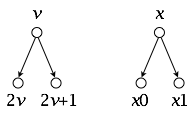
\includegraphics[scale=0.5]{FiguresGraph/codingTree1}
\caption{The graph-theoretic action of one application of the functions $F_0$ and $F_1$:
(left) when the vertices of $\g(\N^+; F_0, F_1)$ are viewed as integers; (right) when the vertices
are viewed as bit-strings.}  
\label{fig:one-node-tree}
\end{center}
\end{figure}
The figure depicts just one tree-vertex and its children.  In the system as described, every vertex is a positive integer, and the arcs are generated by the functions $F_0$ and $F_1$; when recast into ``string-label mode", every vertex is a binary string, and the arcs are generated by the functions ``append $0$" and ``append $1$".

\bigskip

\noindent {\it 2. The root-looped directed infinite binary tree.}
For reasons that will become clear in the upcoming paragraph 3, we amend the just-described
system so that it generates a ``cousin" of the directed infinite binary tree.  A ``prefix" of this tree appears in Fig.~\ref{fig:TreeLabelling}.
\begin{figure}[hbt]
\begin{center}
       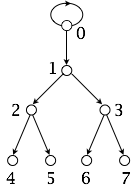
\includegraphics[scale=0.5]{FiguresGraph/TreeLabelling}
\caption{The root-looped $7$-vertex complete binary tree with special vertex $0$.}
\label{fig:TreeLabelling}
\end{center}
\end{figure}
This cousin is the tree with a special vertex, call it $r$; vertex $r$ has two emerging arcs (as do all vertices): One of the new arcs is a {\em self-loop} on $r$; the other points to the root of the directed infinite binary tree of paragraph 1.  One generates the cousin by:
\begin{itemize}
\item
using the set $\N$ of {\em nonnegative} integers as vertices, instead of the earlier-used set $\N^+$ of {\em positive} integers;
\medskip\item
using the same functions $F_0$ and $F_1$ to generate the arcs of the new graph.

\smallskip

Of course, $F_0$ and $F_1$ now have an extended domain, but their ``action" is unchanged: $F_0(x) = 2x$ and $F_1(x) = 2x+1$.
\end{itemize}
In the new digraph, vertex $0$ is the special vertex $r$.  The {\em self-loop} on vertex $r=0$ occurs because $F_0(0) = 2 \times 0 = 0$.  The remainder of this new digraph is the directed infinite binary tree of paragraph 1.

\bigskip

\index{de Bruijn graph/network!algebraic representation}
\noindent {\it 3. The de Bruijn network as the Escherian root-looped directed infinite binary tree.}
We derive the desired connection between the tree-like digraph of paragraph 2 and the order-$n$
de Bruijn network by presenting the latter digraph algebraically, specifically, as the system 
\[ \g(\{0, 1, \ldots, 2^n-1\}; F^{(n)}_0, F^{(n)}_1) \]
where
\[ F^{(n)}_0(v) \ = \ 2v \bmod 2^n \ \ \ \ \mbox{ and } \ \ \ \ F^{(n)}_1(v) \ = \ 2v +1 \bmod 2^n \]
The system $\g(\{0, 1, \ldots, 2^n-1\}; F^{(n)}_0, F^{(n)}_1)$ thus differs from the infinite system 
$\g(\N; F_0, F_1)$---which generates the root-looped directed infinite binary tree---by truncating
both the set of vertices (by keeping only the first $2^n$ nonnegative integers) and the arc-generators.  The truncation is achieved by reducing all integers modulo $2^n$.  See Fig.~\ref{fig:deBruijn}.
\begin{figure}[hbt]
\begin{center}
       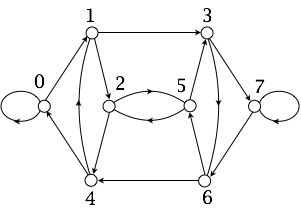
\includegraphics[scale=0.5]{FiguresGraph/dB2by3numbers}
       \caption{A standard depiction of $\d_3$, with vertex-names being the integers corresponding to the usual binary string-labels.}
  \label{fig:deBruijn}
\end{center}
\end{figure}

\smallskip

To see that the system $\g(\{0, 1, \ldots, 2^n-1\}; F^{(n)}_0, F^{(n)}_1)$ is, in fact, the order-$n$
de Bruijn network, let us observe what the functions $F^{(n)}_0$ and $F^{(n)}_1$ do to an
argument integer/vertex $v$.
\begin{itemize}
\item
The {\em number-related} specification
\[ v \ \longrightarrow \ 2v \bmod 2^n \]
corresponds to the {\em numeral-related} specification
\[ \beta x \ \longrightarrow \ x0 \]
where $\beta \in \{0,1\}$ and $x$ is a length-$(n-1)$ bit-string.

\item
The {\em number-related} specification
\[ v \ \longrightarrow \ 2v+1  \bmod 2^n \]
corresponds to the {\em numeral-related} specification
\[ \beta x \ \longrightarrow \ x1 \]
where $\beta \in \{0,1\}$ and $x$ is a length-$(n-1)$ bit-string.
\end{itemize}
The system $\g(\{0, 1, \ldots, 2^n-1\}; F^{(n)}_0, F^{(n)}_1)$ thus specifies the local
graph-theoretic structure depicted in Fig.~\ref{fig:one-DB-node}.
\begin{figure}[hbt]
\begin{center}
       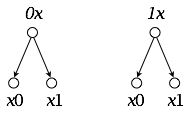
\includegraphics[scale=0.5]{FiguresGraph/codingTree2}
\caption{The graph-theoretic action of one application of the arc-generating functions 
$F^{(n)}_0$ and  $F^{(n)}_1$ to vertices of the forms $x0$ (left) and $x1$ (right).}
\label{fig:one-DB-node}
\end{center}
\end{figure}
A look back at Section~\ref{sec:deBruijn} will verify that the system
$\g(\{0, 1, \ldots, 2^n-1\}; F^{(n)}_0, F^{(n)}_1)$ is, in fact, (isomorphic to) $\d_n$.

\vspace*{.35in}

One often reads about connections between mathematics and art.  It is probably fair to predict that the connection we have just revealed is not what most references to a mathematics-art nexus are referring to.  But there it is!


\ignore{***********
\[
\begin{array}{|ccccccc|}
\hline
\multicolumn{3}{c}{\mbox{Arc-labels: Tree}} & \hspace*{.2in}& \multicolumn{3}{c}{\mbox{Arc-labels: De Bruijn network}} \\
\hline 
F_0(x) & = & 2x      &  &  F^{(n)}_0(x) & = & 2x \bmod 2^n \\
F_1(x) & = & 2x+1  &  &  F^{(n)}_1(x) & = & 2x +1 \bmod 2^n \\ 
\hline
\end{array}
\]

\[
\begin{array}{|c|ccccc|}
\hline
\mbox{vertex} & \multicolumn{2}{c}{\mbox{Tree-successor}} & \hspace*{.2in} & \multicolumn{2}{c}{\mbox{de Bruijn-successor}} \\
\hline
v & F_0(v) & F_1(v) & & F^{(n)}_0(v))& F^{(n)}_1(v) \\
\hline
0 & 0 & 1 & & 0 & 1 \\ 
1 & 2 & 3 & & 2 & 3 \\
2 & 4 & 5 & & 4 & 5 \\
3 & 6 & 7 & & 6 & 7 \\
4 & \cdots & \cdots  & & 0 & 1 \\
5 & \cdots & \cdots  & & 2 & 3 \\
6 & \cdots & \cdots  & & 4 & 5 \\
7 & \cdots & \cdots  & & 6 & 7 \\
\hline
\end{array}
\]
***************}
